\chapter{ΑΝΑΣΚΟΠΗΣΗ ΤΩΝ ΑΡΘΡΩΝ}

\section{ΠΡΟΣΕΓΓΙΣΕΙΣ ΜΕ ΒΑΣΗ ΤΗΝ XML}
    Το άρθρο "\textit{XML-based approaches for the integration of heterogeneous bio-molecular data}" των Mesiti, Jimenez-Ruiz κ.α. πραγματεύεται κάποιες προσεγγίσεις για την αναπαράσταση, ενσωμάτωση και διαχείριση βιολογικών δεδομένων με τη χρήση της XML γλώσσας και άλλων παρεμφερών υλοποιήσεων.
    Επιπλέον, παρουσιάζεται μια νέα προσέγγιση για τη διαχείριση ετερογενών βιολογικών δεδομένων μέσω της XML. \cite{XMLbasedApproaches}
    
    \subsection{Χρησιμότητα XML}
        Η XML έχει αναδειχθεί ως την πιο αποτελεσματική πρόταση για την αναπαράσταση δομημένων πληροφοριών, μιας και επιτρέπει την εύκολη επέκταση και τροποποίηση, κάτι βολικό μιας και καθημερινά δημιουργούνται νέα βιολογικά δεδομένα.
        Υποστηρίζεται από γλώσσες ερωτημάτων (query languages) όπως η XPath και XQuery, δίνοντας τη δυνατότητα για άμεση εξόρυξη των πληροφοριών.

        Χρησιμοποιεί μια ιεραρχική δόμηση της πληροφορίας με στοιχεία (XML Elements), xαρακτηριστικά (XML attributes) και κείμενο (XML text content).
        Κάθε στοιχείο μπορεί να αναπαριστά κάποια συγκεκριμένη βιολογική οντότητα (πχ DNA, RNA, πρωτεΐνη) και μπορεί να περιλαμβάνει εμφωλευμένα στοιχεία για συσχετιζόμενα χαρακτηριστικα.
        Αυτή η ιεραρχική δόμηση αναπαριστά με σαφήνεια πολύπλοκες βιολογικές σχέσεις.


    \subsection{Βιολογικοί τύποι δεδομένων}
        Το άρθρο παρουσιάζει κάποιους τύπους βιολογικών δεδομένων. Για παράδειγμα:
    \begin{itemize}[label={\tiny \blacksquare}]
        \vspace{-10pt}
        \item \textbf{Δεδομένα πρωτοταγών πρωτεϊνών}: περιλαμβάνουν δεδομένα νουκλεοτιδικών αλληλουχιών, φιλοξενούνται σε βάσεις δεδομένων όπως GenBank και EMBL.
        \item \textbf{Δεδομένα πρωτεϊνών}: βάσεις δεδομένων όπως SWISSPROT και TREMBL περιέχουν πληροφορίες για πρωτεϊνικές αλληλουχίες, αναπαρίστανται εύκολα σε XML.
        \item \textbf{Motif (μοτίβα) και πρωτεϊνικές περιοχές}: προσδιορίζονται μέσω μεθόδων αναγνώρισης προτύπων που εφαρμόζονται σε δεδομένα πρωτοταγών πρωτεϊνών, αναπαρίστανται με μια περιγραφή του μοτίβου, βιβλιογραφικές πληροφορίες κ.α.
    \end{itemize}

    \subsection{Αναπαράσταση βιολογικών δεδομένων με τη χρήση XML}
        Έχουν χρησιμοποιηθεί αρκετές γλώσσες βασισμένες στην XML, ειδικά για την αναπαράσταση διαφορετικών τύπων βιολογικών δεδομένων. Για παράδειγμα:

        \subsubsection{Bioinformatic Sequence Markup Language (BSML)}
            Γλώσσα σχεδιασμένη για να περιγράφει αλληλουχίες όπως DNA, RNA και πρωτεϊνικές αλληλουχίες.
            Ένα BSML αρχείο περιλαμβάνει πληροφορίες για το πώς τα γονιδιώματα κωδικοποιούνται, ανακτώνονται και εμφανίζονται.

        \subsubsection{Protein Markup Language - ProXML}
            Χρησιμοποιείται για την αναπαράσταση πρωτεϊνικών αλληλουχιών.
            Περιλαμβάνει ένα identity section που περιέχει την περιγραφή των πρωτεϊνών και ένα data section που περιέχει ιδιότητες από αυτές τις πρωτεΐνες.

        \subsubsection{ΠΡΟΕΚΤΑΣΗ: RNA Markup Language - RNAML}
            Γλώσσα που σχεδιάστηκε με σκοπό να διευκολύνει την ανταλλαγή RNA πληροφοριών μεταξύ διαφορετικών λογισμικών βιοπληροφορικής. \cite{RNAML}
            Μέχρι πρότινος, κάθε εργαστήριο ανέπτυσσε το δικό του λογισμικό με τους δικούς του τύπους αρχείων για την ανάγνωση και την εγγραφή της βιοπληροφορίας.
            Επομένως, κατέστη αναγκαία η δημιουργία μιας τυποποιημένης σύνταξης της RNA πληροφορίας, η οποία έχει σκοπό να αυξήσει την αποτελεσματικότητα στην κοινότητα των βιολόγων.

            Οι προηγούμενες προσπάθειες για τυποποίηση της βιολογικής πληροφορίας περιλαμβάνουν την BIOpolymer Markup Language (BIOML) γλώσσα σήμανσης, η οποία αναπτύχθηκε το 1999 από την ProteoMaterics.
            Περιλαμβάνει ένα διευρυμένο framework για τον καθορισμό μοριακών οντοτήτων, και ενώ περιλάμβανε κάποιες πληροφορίες για το RNA, εστιάζονταν περισσότερο στη γονιδιακή του πλευρά (θέσεις έναρξης και παύσης της μεταγραφής και γενετικές τροποποιήσεις).
            Δεν κάλυπτε επαρκώς πληροφορίες για τη δομή του RNA, κάτι ερευνητικά κρίσιμο.
            Επομένως, δεν κάλυπταν τις απαιτήσεις που έθετε η επιστημονική κοινότητα που μελετούσε το RNA, οδηγώντας στην ανάπτυξη της RNAML.

            Η RNAML βασίζεται πάνω στο XML.
            Υπάρχει η δυνατότητα δημιουργίας ενός Document Type Definition (DTD) το οποίο καθορίζει τη δομή του εγγράφου, τα ονόματα και τον τύπο των στοιχείων και τη ιεραρχική δομή τους, κάτι που διασφαλίζει τη συνέπεια και τη συμμόρφωση στο πώς αναπαρίσταται το RNA.
            Επίσης, αναπαριστά πληροφορία για την αλληλεπίδραση πολλαπλών μορίων RNA, την απόσταση τους, τη σύζευξη των βάσεών τους, και οποιαδήποτε άλλη σχέση έχουν μεταξύ τους.
            Τέλος, πέρα από δυνατότητες για σχολιασμό και documentation σε κάθε στοιχείο, είναι δυνατή η ομαδοποίηση των εμφανίσεων του ίδιου λειτουργικού RNA σε διαφορετικούς οργανισμούς, επιτρέποντας την αναπαράσταση ευθυγραμμίσεων και κοινών δομικών συστατικών.

        \subsubsection{ΠΡΟΕΚΤΑΣΗ: System Biology Markup Language (SBML)}
            Δημιουργήθηκε στα πλαίσια του ERATO Kitano Systems Biology Project για να διευκολύνει την ανταλλαγή μοντέλων μεταξύ διαφορετικών εργαλείων προσομοίωσης και ανάλυσης. \cite{SBML}

            Ένα SBML μοντέλο περιλαμβάνεται από το Διαμέρισμα (Compartment), έναν καθορισμένο χώρο όπου συμβαίνουν οι αντιδράσεις όπως ένα κύτταρο ή ένα οργανίδιο,
                ένα Eίδος (Species), οι χημικές οντότητες που συμμετέχουν στις αντιδράσεις όπως τα ιόντα ή τα μόρια, η Αντίδραση (Reaction), η διαδικασία σχηματισμού μεταξύ των ειδών,
                η Παράμετρος (Parameter), όπου αναπαριστά ποσότητες με συμβολικά ονόματα τοπικά η καθολικά, Ορισμοί Μονάδων (Unit Definitions), για τον προσδιορισμό των μονάδων που χρησιμοποιούνται στο μοντέλο,
                και τέλος οι Κανόνες (Rules), μαθηματικές εκφράσεις που ορίζουν τις τιμές των παραμέτρων ή θέτουν περιορισμούς στο μοντέλο.

            \begin{figure}[ht] \noindent\centering
                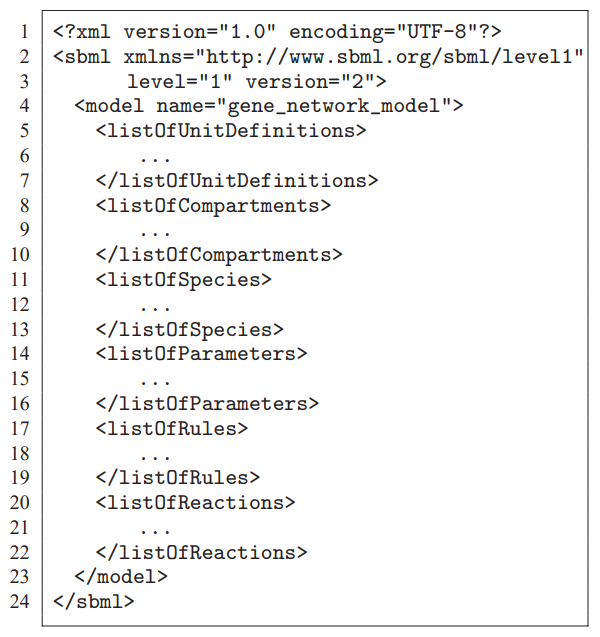
\includegraphics[scale=0.7]{img/SBML skeleton}
                \caption{Σκελετός από τον ορισμό ενός μοντέλου \cite{SBML}}
            \end{figure}

        \subsubsection{ΠΡΟΕΚΤΑΣΗ: Cell Markup Language (CellML)}
            Το CellML προσφέρει μια σαφή μέθοδο ορισμού μοντέλων κυτταρικής λειτουργίας, σε ένα πιο γενικό πλαίσιο σε σχέση με τα προηγούμενα. \cite{CellML}
            Το βάθος στο οποίο μπορεί το CellML να αναπαραστήσει τις έννοιες επικαλύπτει γλώσσες όπως η SBML, με τη διαφορά ότι η SBML βασίζεται περισσότερο στην περιγραφή βιοχημικών αντιδράσεων, χάνοντας πληοροφορία για τη δομή των μοντέλων.

            Η CellML από την αρχή σχεδιάστηκε για να υποστηρίξει μοντέλα μεγάλης κλίμακας, επιτρέπεται (λόγω της XML βάσης της) η ανεξάρτητη κατασκευή μοντέλων και τμημάτων και η ενσωμάτωσή τους σε ένα μεγαλύτερο μοντέλο, και παρέχει τρόπους για την απόκρυψη low-level πληροφοριών ώστε να μη συγχέονται με το υψηλότερο επίπεδο αναπαράστασης του μοντέλου.

            \begin{figure}[ht] \noindent\centering
                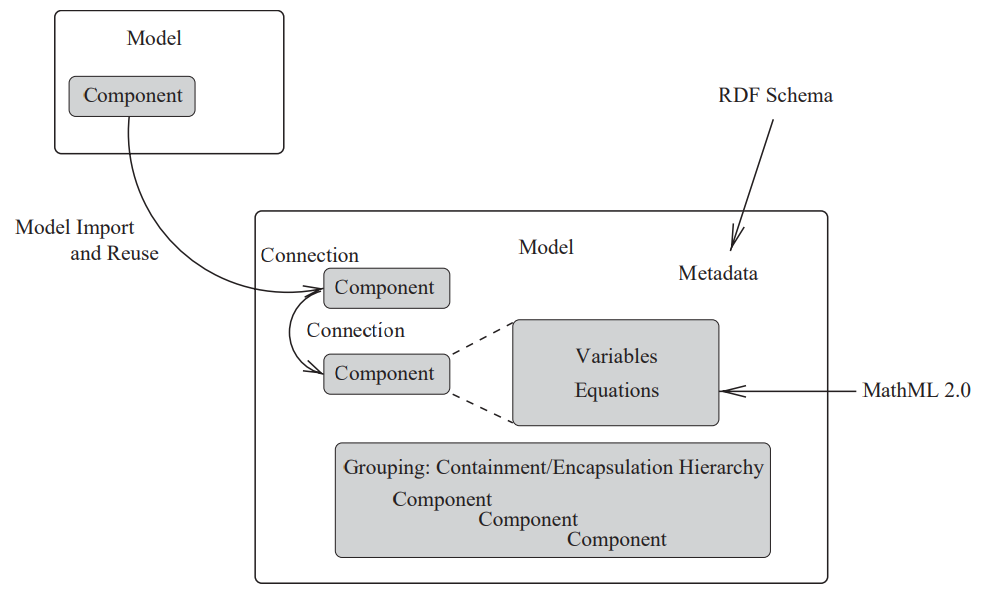
\includegraphics[scale=0.7]{img/CellML structure}
                \caption{Διάγραμμα με το σκελετό ενός CellML μοντέλου \cite{CellML}}
            \end{figure}


    \subsection{Διαχείριση ετερογενών βιολογικών δεδομένων}
        Οι βιολόγοι συνήθως χρησιμοποιούν διαφορετικές βάσεις δεδομένων, η κάθε μία με το δικό της σχεδιασμό της πληροφορίας, που καθιστά χρονοβόρα τη ανάκτηση πληροφορίας.
        Επομένως, είναι αυξημένη η ανάγκη για πρόσβαση σε μια ομογενοποιημένη βάση δεδομένων, κάτι που δεν είναι πάντα εύκολο να επιτευχθεί λόγω της ετερογένειας της πληροφορίας.

        Λύση σε αυτό είναι η γλώσσα XML, που προφέρει έναν τρόπο για τη συντακτική ενσωμάτωση των δεδομένων, αν και στερείται των μεθόδων με τους οποίους μπορεί να επιτευχθεί αυτή η ενσωμάτωση.
        Τέτοιες μέθοδοι ονομάζονται αρχιτεκτονικές ενσωμάτωσης (integration architectures) και χωρίζονται στις Data warehouse, Mediator-based, Service oriented και Peer-based αρχιτεκτονικές.

        Το δεύτερο μέρος του άρθρου αναλύει τη χρήση αυτών των αρχιτεκτονικών σε συνδυασμό με την XML για την ενσωμάτωση των δεδομένων.

% έχω μείνει στο Integration aspects
